% Select language used in document (ngerman or english). Automatically
% generated text is translated accordingly.
% use \selectthesislanguage in body.tex to switch to default language

%\documentclass[ngerman, paper]{mmt} % use for seminar paper
%\documentclass[ngerman, reviewversion]{mmt} % use for anonymized review version 
%\documentclass[ngerman, bachelorthesis]{mmt} % use for Bachelor thesis
\documentclass[ngerman, masterthesis]{mmt} % use for Master thesis

\usepackage{mathptmx}
\usepackage{graphicx}
\usepackage{times}
\usepackage{subfig}
\usepackage{float}
\usepackage[utf8]{inputenc}
\usepackage{listings}
\usepackage{makecell}
\usepackage[toc,page]{appendix}
\usepackage{hyperref}
\hypersetup{
    colorlinks,
    citecolor=black,
    filecolor=black,
    linkcolor=black,
    urlcolor=black
}
\usepackage{breakurl}

\usepackage{amsmath}
\usepackage[autostyle,german=guillemets]{csquotes}

% moved to cls file. use \selectthesislanguage to switch to default language
%\usepackage[english,ngerman]{babel}

\usepackage{abbrevs}
%% the following solves a bug in the abbrevs package, that adds an empty
%% space after the abbrev
\makeatletter
\renewcommand\maybe@space@{%
  % \@tempswatrue % <= this is in the original
  \maybe@ictrue % <= this is new
  \expandafter   \@tfor
    \expandafter \reserved@a
    \expandafter :%
    \expandafter =%
                 \nospacelist
                 \do \t@st@ic
  % \if@tempswa % <= this is in the original
  \ifmaybe@ic % <= this is new
    \space
  \fi
}
\makeatother
%%


\usepackage{listings}
\usepackage{color}
\definecolor{lightgray}{rgb}{.9,.9,.9}
\definecolor{darkgray}{rgb}{.4,.4,.4}
\definecolor{purple}{rgb}{0.65, 0.12, 0.82}
\lstdefinelanguage{JavaScript}{
  keywords={break, case, catch, continue, debugger, default, delete, do, else, false, finally, for, function, if, in, instanceof, new, null, return, switch, this, throw, true, try, typeof, var, let, const, void, while, with},
  morecomment=[l]{//},
  morecomment=[s]{/*}{*/},
  morestring=[b]',
  morestring=[b]",
  ndkeywords={class, export, boolean, throw, implements, import, this},
  keywordstyle=\color{blue}\bfseries,
  ndkeywordstyle=\color{darkgray}\bfseries,
  identifierstyle=\color{black},
  commentstyle=\color{purple}\ttfamily,
  stringstyle=\color{red}\ttfamily,
  sensitive=true
}

\lstset{
   language=JavaScript,
   backgroundcolor=\color{lightgray},
   extendedchars=true,
   basicstyle=\footnotesize\ttfamily,
   showstringspaces=false,
   showspaces=false,
   numbers=left,
   numberstyle=\footnotesize,
   numbersep=9pt,
   tabsize=2,
   breaklines=true,
   showtabs=false,
   captionpos=b
}

\usepackage[authordate,bibencoding=auto,strict,noibid,backend=biber]{biblatex-chicago}
\bibliography{bibliography}

%% Add configuration options
\newabbrev{\authorname}{Bernhard Schmidhuber}
\newabbrev{\authormail}{bschmidhuber.mmt-b2019@fh-salzburg.ac.at}
\newabbrev{\titlename}{Guarantees for spectral clustering with fairness constraints}
\newabbrev{\advisor}{Dr. Simon Ginzinger}
\newabbrev{\thesisdate}{12.05.2021}
\newabbrev{\thesisrepo}{https://github.com/BSchmidhuber/fhs-sem4-seminararbeit}
\newabbrev{\keywordsenglish}{spectral, clustering, fairness, constraints, grouping, algorithms}


%% Paper title.

\title{\titlename}

%% This is how authors are specified in the conference style

%% Author 
\author{ \authorname\\ \scriptsize \authormail \\ \scriptsize 
\ifmmtlanguagegerman FH Salzburg \else Salzburg University of Applied Sciences \fi
}

%% A teaser figure can be included as follows, but is not recommended since
%% the space is now taken up by a full width abstract.
%\teaser{
%  \includegraphics[width=1.5in]{sample.eps}
%  \caption{This can be a teaser image of the thesis.}
%}

%% Abstract section for paper format.
\abstract{
    \ifmmtlanguagegerman 
        \selectlanguage{ngerman}
        Am Anfang wurde das Universum erschaffen. Das störte viele Leute und wurde
generell als schechte Idee betrachtet.
    \else 
        \selectlanguage{english}
        The importance of fairness constraints in the clustering domain of unsupervised learning has been increasing in recent years. Since there are already various papers on the algorithms used for this purpose, this paper aims to provide an overview of the possibilities to add fairness constraints in different clustering algorithms. After a clarification of important terms, definitions and concepts, the known algorithms for $k$-center, $k$-means and spectral clustering are explained and the possible fairness constraints are shown and compared.
    \fi
}

%%%%%%%%%%%%%%%%%%%%%%%%%%%%%%%%%%%%%%%%%%%%%%%%%%%%%%%%%%%%%%%%
%%%%%%%%%%%%%%%%%%%%%% START OF THE PAPER %%%%%%%%%%%%%%%%%%%%%%
%%%%%%%%%%%%%%%%%%%%%%%%%%%%%%%%%%%%%%%%%%%%%%%%%%%%%%%%%%%%%%%%%

\begin{document}
% TODO switch for english, german
\selectthesislanguage

\pagenumbering{gobble}

 % group open
\ifmmtpaper
    \begingroup 
    % is required because paper template messes with sizes
    \fontsize{12}{18}\selectfont        
    \setlength{\parindent}{0pt}
    \setlength{\parskip}{5pt plus 2pt minus 1pt}
    \sectionfont{\fontsize{14}{15}\selectfont}
\fi

\ifmmtreviewversion\else
    \begin{titlepage}

% check if second advisor exists
\newcommand{\printsecondadvisor}[1]{%
  \ifcsname#1\endcsname%
  \ifmmtlanguagegerman ZweitbetreuerIn: \else Second Advisor: \fi \secondadvisor 
  \else%
    
  \fi%
}

\ifmmtmasterthesis

    
    % \begin{center}
    %     \Huge{ 
    %     	\textbf{\ifmmtlanguagegerman Masterarbeit \else Master Thesis \fi}
    %     }
    % \end{center}
    
    \newpage
    
    \thispagestyle{empty}
    
    \hfill \includegraphics[height=1.5cm]{images/FHSLogo.jpg}
    
    \vspace*{2cm}
    
    \Large{
    \titlename
    
    \vspace*{1cm}
    
    \ifmmtlanguagegerman
    Masterarbeit zur Erlangung des akademischen Grades
    \else
    Master thesis in partial fulfilment of the requirements for\\ the degree of 
    \fi
    
    \vspace*{0.5cm}
    
    \textit{Master of Science}
    }
    
    
    \vspace*{1.5cm}
    {\large
    \ifmmtlanguagegerman AutorIn: \else Author: \fi \authorname
    }
    \vfill
    
    {\normalsize
    \ifmmtlanguagegerman
    Vorgelegt am FH-Masterstudiengang MultiMediaTechnology, Fachhochschule Salzburg
    \else
    Submitted to the Master degree program MultiMediaTechnology, Salzburg University of Applied Sciences
    \fi
    
    
    \vspace*{1cm}
    
    \ifmmtlanguagegerman BetreuerIn: \else Advisor: \fi
    \advisor
    \\    
    \printsecondadvisor{secondadvisor}
    
    \vfill
    
    Salzburg, \ifmmtlanguagegerman Österreich, \else Austria, \fi  \thesisdate
    }

\else % Bachelor thesis title page

    \begin{center}
    
    \includegraphics[width=5cm]{images/FHSLogo.jpg}


    \vspace*{4cm}
    
    \fontsize{20.79}{18pt}{\selectfont        
    %\Large{
    	\textit{\textbf{\titlename}}
    %}
    }
    
    \vspace*{4cm}
    
    \fontsize{20.79}{18pt}{%\large{
    \ifmmtlanguagegerman
      \textbf{ \ifmmtpaper Seminararbeit \else Bachelorarbeit \fi }
    \else
        \textbf{ \ifmmtpaper Seminararbeit \else Bachelor Thesis \fi }
    \fi
    }
    
    
    \end{center}
    
    \vfill
    
    %\begin{tabular}{ll}
    \ifmmtlanguagegerman AutorIn: \else Author: \fi  \authorname  \\
    \ifmmtlanguagegerman BetreuerIn: \else Advisor: \fi \advisor \\
    \printsecondadvisor{secondadvisor}
    
    Salzburg, \ifmmtlanguagegerman Österreich, \else Austria, \fi \thesisdate
    
    
    
    % uncomment the following 3 lines for an optional lock flag, max. 2 years!
    %\hfill
    %\color{red}
    %\framebox{Sperrvermerk bis 20/01/2012}

\fi

\end{titlepage}
       
\fi

    \onecolumn           
    
    \pagenumbering{roman}
    
\ifmmtpaper % does not need affidavit
\else \ifmmtreviewversion
      \else
        \newpage
        \input{affidavit}  % comment out for expose
      \fi
\fi
% group closing
\ifmmtpaper
\endgroup
\fi


\ifmmtpaper \else \ifmmtreviewversion\else  % paper does not need this stuff
    
    \newpage
    \selectlanguage{ngerman}
    \section*{Kurzfassung}
    Am Anfang wurde das Universum erschaffen. Das störte viele Leute und wurde
generell als schechte Idee betrachtet.
    \ifmmtmasterthesis
    
    \vspace*{0.5cm} 
    \textbf{Schlüsselwörter:~} \keywordsgerman
    \fi
    \newpage
    \selectlanguage{english}
    \section*{Abstract}
    The importance of fairness constraints in the clustering domain of unsupervised learning has been increasing in recent years. Since there are already various papers on the algorithms used for this purpose, this paper aims to provide an overview of the possibilities to add fairness constraints in different clustering algorithms. After a clarification of important terms, definitions and concepts, the known algorithms for $k$-center, $k$-means and spectral clustering are explained and the possible fairness constraints are shown and compared.
    \ifmmtmasterthesis
        
    \vspace*{0.5cm} 
    \textbf{Keywords:~} \keywordsenglish
    \fi
    \selectthesislanguage
    
    \newpage
    \tableofcontents
    
    \newpage
    \listoffigures
    \lstlistoflistings
    \listoftables
    
\fi
\fi

\mmtcolumnmode % switch back to column formatting of stylesheet

\maketitle % used for paper formatting

\ifmmtpaper\else
\pagestyle{headings}
\fi
\pagenumbering{arabic}


\section{Introduction}

In the last couple of years the topic "fairness" in the area of machine learning has become more and more important. While it was a minor issue in the early years of machine learning, today larger companies like Google have special departments for the topic of fairness in machine learning.

The first paper that focused on this issue was "Fair Clustering Through Fairlets" by \textcite{Chierichetti2018}, it subsequently served as a reference for many other papers in this research area.

The main reason why the topic became so important is that artificial intelligence, of which machine learning is a big part, is now having a huge impact on our daily lives. Whether smart homes, personalized advertisements on the Internet or self-driving cars - artificial intelligence is being used more and more in each of these areas. This also increases the problem that machines are mostly exposed to unbalanced and biased data when they are "learning". This ethical problem also comes with technical challenges.

\begin{quote}
    "Many important decisions today are made by machine learning algorithms. [...] It is important to ensure that such algorithms are fair and are not biased towards or against some specific groups in the population."
\autocite[1]{Bera2019}
\end{quote}

This paper gives a brief overview of three different clustering algorithms in the field of unsupervised learning \autocite[]{Barlow1989}. You will learn the basic differences between \nameref{k-center} \autocite[]{Chierichetti2018}, \nameref{k-means} \autocite[]{Schmidt2018} and \nameref{spectral-clustering} \autocite[]{Kleindessner2019}. We will look at the differences in applying fairness constraints to these algorithms and their implications.
\section{Definitions}


\subsection{Clustering}

When it comes to data analysis in the area of unsupervised machine learning, \textcite[1]{VonLuxburg2007} says that "Clustering is one of the most widely used techniques for exploratory data analysis [...]". For this purpose, data is analyzed so that groups with similar behavior can be identified and summarized.

\textcite[]{Bera2019} sum it up with the addition, that "Clustering is a fundamental unsupervised learning problem where one wants to partition a given data-set. In machine learning, clustering is often used for feature generation and enhancement as well. It is thus important to consider the bias and unfairness issues when inspecting the quality of clusters." \autocite[1]{Bera2019}

"Considerable research in machine learning and pattern recognition" has the focus on "the task of finding good clusters". \autocite[1]{Ng2001}

\textcite[1]{Nascimento2011} add, that "Clustering is an unsupervised technique concerned with the grouping of related objects without taking their class or label into account."

There are various \nameref{clustering-algorithms} that we will have a look at in \autoref{clustering-algorithms}.

\subsubsection{$k$-Clustering}

As  \textcite[]{Chierichetti2018} said, we understand all different types of $k$-clustering as algorithms based on dividing an existing set of points into $k$ subsets. They describe that one has a set $X$ in a $n$-dimensional space, the $k$-clustering $C$ is a partition of $X$ in $k$ disjoint subsets, $C_{1},...,C_{k}$, called Clusters. \autocite[3]{Chierichetti2018}

While the work of \textcite[]{Chierichetti2018} has been about fairness constraints for the \nameref{k-center} and the \hyperref[k-median]{$k$-median} algorithms, \textcite[]{Schmidt2018} have focused on fairness constraints for the \hyperref[k-means]{$k$-means} algorithm.

\subsubsection{Other Clustering Types}

Although there are many different clustering types, like density-based clustering or distribution-based clustering, we focus on one particular algorithm in this paper, which is the \nameref{spectral-clustering}.

\textcite[]{Kleindessner2019} had their focus on fairness constraints for \nameref{spectral-clustering}.


\subsection{Fairness}

To define fairness in the area of machine learning \textcite[1]{Kleindessner2019} said, that "[...] a clustering is fair if every demographic group is approximately proportionally represented in each cluster."

\textcite[1]{Feldman2014CertifyingImpact} raises the question of biased algorithms and claims that "unintentional bias" is called "disparate impact, which occurs when a selection process has widely different outcomes for different groups, even as it appears to be neutral." There is a problem of "determining disparate impact", especially "when computers are involved".


\section{Concepts and Techniques}


\subsection{Fairlets}
\label{fairlets}

The first concept presented in this paper is the concept of fairlets. The term "fairlet" was introduced by  \textcite[]{Chierichetti2018}, to denote "minimal sets that satisfy fair representation
while approximately preserving the clustering objective." \autocite[1]{Chierichetti2018}

\subsubsection{Balance}

To understand the concept of fairlets, it is first necessary to understand the concept of balance. Assuming we have a data set of red and blue data points, balance is the quotient of the smaller by the larger value, which must be between 0 and 1. If we have a completely balanced distribution of data points, e.g. 5 red and 5 blue points, the balance is 1, which means that the data set is perfectly balanced. If it is relatively unbalanced, e.g. 1 red data point and 10 blue, the balance is $\frac{1}{10}$ = 0.1. If we don't have any points at all from one color, the balance is 0, so fully unbalanced. This balance can also be combined in disjoint subsets by using the minimum balance of each case, which provides a basis for the concept of fairlets. \autocite[4]{Chierichetti2018}

\begin{quote}
"Balance encapsulates a specific notion of fairness, where a clustering with a monochromatic cluster (i.e., fully unbalanced) is considered unfair."

\autocite[4]{Chierichetti2018}
\end{quote}

\subsubsection{Fairlet decomposition}

Once the balance has been determined, a clustering can be constructed iteratively from the original data set. For that, single data points are removed as long as the balance between the remaining data points can be kept the same. To bring fairness into play, this process to get a minimum data set with the same balance is called fairlet decomposition, because the so-called ($t, k$)-fairlets are decomposed until you get $k$ desired clusters that have reached a corresponding balance of $t$. \autocite[4]{Chierichetti2018}

Finally, \textcite[4]{Chierichetti2018} state that "balance encapsulates a specific notion of fairness, where a clustering with a monochromatic cluster (i.e., fully unbalanced) is considered unfair. So we call the clustering [...] a $(b, r)$\textit{-fairlet decomposition} [...] and call each cluster [...] \textit{a fairlet}." \autocite[4]{Chierichetti2018}


\subsection{Stochastic Block Models}

Stochastic Block Models were introduced and defined by \textcite[]{Holland1983}:

\begin{quote}
"A stochastic model is proposed for social networks in which the actors in a network are partitioned into subgroups called blocks. The model provides a stochastic generalization of the blockmodel."

\autocite[1]{Holland1983}
\end{quote}

\textcite[1]{Karrer2010StochasticNetworks} describe it as a "generative model for blocks, groups, or communities in networks." Classified as "random graph models" they already exist for a long time in the area of computer science.
The simplest form of a stochastic block model is that "each of $n$ vertices is assigned to one of $K$ blocks, groups, or communities, and undirected edges are placed independently between vertex pairs with probabilities that are a function only of the group memberships of the vertices." \autocite[1]{Karrer2010StochasticNetworks}

In the case of clustering, \textcite[]{Lei2013} describe the consistency of spectral clustering in stochastic block models. They "show that, under mild conditions, spectral clustering applied to the adjacency matrix of the network can consistently recover hidden communities even when the order of the maximum expected degree is as small as log $n$, with $n$ the number of nodes." \autocite[1]{Lei2013}

\section{Clustering Algorithms}
\label{clustering-algorithms}


\subsection{$k$-center}
\label{k-center}

\subsubsection{General}
The $k$-center clustering is a problem that is categorized as "NP-hard" (= non-deterministic polynomial-time hard), which means that it is very likely that there never will be efficient algorithms to solve that problem. Therefore, you need to resort to approximation algorithms.
For example, there is a "greedy algorithm" by \textcite[]{Gonzalez1985ClusteringDistance} which can solve the problem of NP-hardness.

This $k$-center algorithm consists of a parameter $k$, which defines the number of center points, and a set of center points $C$, where $c_{1},...,c_{k}$ are the so-called centers. \autocite[]{Kleindessner2019FairSummarization}
The greedy strategy by \textcite[]{Gonzalez1985ClusteringDistance} picks an arbitrary element of the data set as the first center point $c_{1}$, calculates the distance for every point in the data set and picks the point with the highest distance as next center point $c_{2}$. At the same time, the center points are optimized iteratively, so the points selected at the beginning are not immediately adopted as a fixed solution. This process of picking and optimizing will be continued until $k$ center points are found.

\subsubsection{Fairness}

\textcite[]{Chierichetti2018} use the concept of \nameref{fairlets} to achieve fairness for $k$-center. In their work, they have two different approaches: the $(1,1)$-fairlets and the $(1,t')$-fairlets.

To find a perfectly balanced clustering, \textcite[]{Chierichetti2018} show an example of a good $(1, 1)$-fairlet decomposition. They stated that "an optimal $(1, 1)$-fairlet decomposition for $k$-center can be found in polynomial time." \autocite[6]{Chierichetti2018} So they proved that they can remove the NP hardness of the algorithm in this case. The big disadvantage of this algorithm, however, is that this insistence on perfect balance or fairness makes the clustering itself correspondingly weaker.

Therefore, it requires a smarter algorithm that brings relatively good fairness without pushing too much on the quality cost of the clustering. \textcite[]{Chierichetti2018} show that in the approach with the $(1,t')$-fairlets, in which they use a clustering with balance $t < 1$ instead. So it is assumed that $t = \frac{1}{t'}$, where $t'$ is an integer value $> 1$. \autocite[6]{Chierichetti2018} With this small adjustment, they no longer assume perfect balance, which increases the strength of the algorithm because cost is also taken into account.


\subsection{$k$-means}
\label{k-means}

\subsubsection{General}

"The global $k$-means clustering algorithm" was introduced by \textcite[]{Likas2003}. They explain that their algorithm "is an incremental approach to clustering that dynamically adds one cluster center at a time through a deterministic global search procedure consisting of $N$ (with $N$ being the size of the data set) executions of the $k$-means algorithm from suitable initial positions." \autocite[1]{Likas2003}

In detail, \textcite[2]{Likas2003} explain the $k$-means algorithm with a given "data set $X = \{x_{1},...,x_{N}\},x_{n} \in \mathbb{R}^d$". Then they try to partition "this data set into $M$ disjoint subsets (clusters) $C_{1},...,C_{M}$" to aim the so-called $M$-clustering problem, "such that a clustering criterion is optimized." They add, that "The most widely used clustering criterion is the sum of the squared Euclidean distances between each data point $x_{i}$ and the centroid $m_{k}$ (cluster center) of the subset $C_{k}$ which contains $x_{i}$. This criterion is called clustering error and depends on the cluster centers $m_{1},...,m_{M}$, [...] where $I(X) = 1$ if $X$ is true and $0$ otherwise."

\subsubsection{Fairness}

\textcite[]{Chierichetti2018} had a look at the fairness approach for the $k$-median clustering algorithm, which is basically an extension for the $k$-means algorithm with the only difference, that it uses the median instead of the mean in each dimension. \autocite[]{Jain1988} This small difference does not affect us further in our analysis, especially since the results for \nameref{k-center} can in principle also be adopted for $k$-median or $k$-means and only minor adjustments are necessary.

\begin{quote}
"Unlike, the $k$-center case, our goal is to find a perfect matching of minimum total cost, since that exactly represents the cost of the fairlet decomposition."
\autocite[9]{Chierichetti2018}
\end{quote}

\textcite[]{Chierichetti2018} have put forward the theorem that "the algorithm that first finds fairlets and then clusters them is a $(2 + \sqrt{3} + \epsilon)$-approximation for the (1, $k$)-fair median problem", which is equivalent to the $(1, 1)$-fairlets example at \nameref{k-center}. For the $(1,t')$-fairlets in the \nameref{k-center}, this can be also modified for approximations like $(t' + 1 + \sqrt{3} + \epsilon)$ for the $(\frac{1}{t'}, k)$-fair median problem. \autocite[9]{Chierichetti2018}

For the basic $k$-means clustering algorithm, \textcite[]{Schmidt2018} wanted to get another solution, because they discovered that "previous algorithms for fair clustering do not scale well." So they came up with a solution of "coresets for fair clustering problems", especially for the $k$-means algorithm, where they are showing how to model and how to compute them. These coresets behave similarly to fairlets and should be there to be able to drastically reduce the size of the input data. They have proven that these coresets can also be easily put together and they also show the possibility of computation in a streaming environment. \autocite[1]{Schmidt2018} 


\subsection{Spectral Clustering}
\label{spectral-clustering}

\subsubsection{General}

When it comes to the spectral clustering method for cluster analysis, the work of \textcite[]{VonLuxburg2007}  "A Tutorial on Spectral Clustering" is a good place to start. It defines this method of clustering as follows:

\begin{quote}
"Compared to the “traditional algorithms” such as $k$-means or single linkage, spectral clustering has many fundamental advantages. Results obtained by spectral clustering often outperform the traditional approaches, spectral clustering is very simple to implement and can be solved efficiently by standard linear algebra methods."
\autocite[1]{VonLuxburg2007}
\end{quote}

Spectral clustering is based on so-called similarity graphs. These show similarities between different data points in an undirected graph $G = (V,E)$. The data is divided into groups: data points in the same group are similar, points in diverse groups are different. \autocite[2]{VonLuxburg2007}

As \textcite[2]{Kleindessner2019} summarize for creating an algorithm for unnormalized spectral clustering, a weighted adjacency matrix is calculated from the similarity graph, and subsequently the Laplacian matrix of it. Then the $k$ smallest eigenvalues of the Laplacian matrix and the corresponding orthonormal eigenvectors are computed. A $k$-means clustering is then applied to this.

While \textcite[]{Kleindessner2019} mainly deal with unnormalized spectral clustering, there are two known variants of normalized spectral clustering by \textcite[]{Shi2000} and \textcite[]{Ng2001}.

\begin{quote}
"The success of spectral clustering is mainly based on the fact that it does not make strong assumptions on the form of the clusters. As opposed to $k$-means, where the resulting clusters form convex sets (or, to be precise, lie in disjoint convex sets of the underlying space), spectral clustering can solve very general problems like intertwined spirals."
\autocite[28]{VonLuxburg2007}
\end{quote}

\subsubsection{Fairness}

In addition to the weighted adjacency matrix, the fair algorithm of \textcite[3]{Kleindessner2019} in spectral clustering requires a group $f^{(s)} \in \{0,1\}^n, s \in [h]$. This allows to compute a fairness matrix which is used instead of the Laplace matrix to get a fair spectral clustering. \autocite[3]{Kleindessner2019}

To be able to better demonstrate this, \textcite[4]{Kleindessner2019} showed a variant of the stochastic block model with 4 blocks of graph data (\ref{fig:kleindessner_variant_sbm}), where points in each group have different properties:
\begin{enumerate}
	\item points in the same cluster and group
	\item points not in the same cluster but in the same group
	\item points in the same cluster but not in the same group
	\item points neither in the same cluster, nor in the same group
\end{enumerate}

When you look at \autoref{fig:kleindessner_variant_sbm}, you can see that the clustering $V = C_{1} \dot\cup C_{2}$ is fair, but the clustering $V = V_{1} \dot\cup V_{2}$ would be highly unfair. \autocite[4]{Kleindessner2019}

But why is that? In total, we see here four separated groups of data points in the form of a graph. The red points representing a separate demographic group in the upper half, the blue points of another demographic group in the lower half. Edges between nodes occur very frequently between the top two groups and between the bottom two groups, only minimally fewer edges we can see between the left two groups and the right two groups. Diagonally, meaning between the top right and the bottom left or the top left and the bottom right, there are hardly any connections.

Let us now assume that a clustering algorithm wants to split the given data points into two clusters. An algorithm without any fairness constraints would now presumably form the two clusters $V_{1}$ and $V_{2}$ drawn in, which however corresponds to an exact split between top and bottom, respectively the demographic groups. This is exactly the kind of split we would like to avoid.

A much fairer separation would be to split the data points between left and right, since in these clusters the original ratios between the demographic groups could be maintained.

\begin{figure}
    \centering
    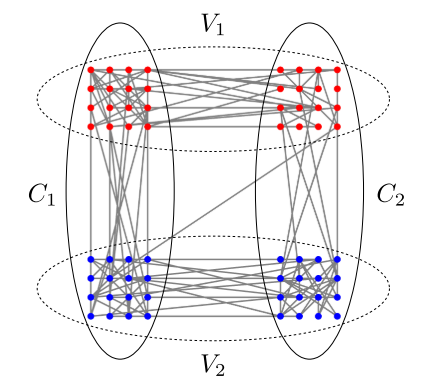
\includegraphics[width=0.9\linewidth]{images/kleindessner_variant_sbm.png}
    \caption{Variant of the Stochastic Block Model of \textcite[4]{Kleindessner2019}}
    \label{fig:kleindessner_variant_sbm}
\end{figure}
\section{Summary and Conclusion}

So you can see that depending on the use case, there are different advantages and disadvantages to which algorithm you should use. Of course, the actually available data set also plays a major role.

Probably the simplest clustering algorithm is the $k$-means algorithm, which tries to keep the variance of the data points within a cluster as small as possible. However, since the algorithm must iterate over all data points, it is recommended that it not be used with extremely large data sets.
In the case of fairness, you have to decide whether you prefer the approach of \textcite{Chierichetti2018} with fairlets, or rather the coresets of \textcite{Schmidt2018}.

The use of the $k$-center algorithm depends very individually on the given data set, or whether well-functioning center points can be found with it.

Spectral clustering does a very good job of representing relatedness and representing specific shapes, such as intertwined spirals. So there again, depending on the available data set, it is key to decide whether spectral clustering is suitable for the particular use case.

The corresponding fairness constraints are very strongly tied to the initial algorithms, which also makes it difficult to compare the different constraints. While $k$-center and $k$-means rely heavily on the concepts of fairlets and coresets, Spectral Clustering has a very simple and clear algorithm that remains very much the same in terms of flow by extending it with a fairness component.

 % the main text

%\input{acknowledgements}

\ifmmtpaper

\printbibliography

\else % only use the following for thesis format

\newpage
\printbibliography

\fi


 % group open
\ifmmtpaper 
\begingroup 
    % is required because paper template messes with sizes
    \fontsize{12}{18}\selectfont        
    \setlength{\parindent}{0pt}
    \setlength{\parskip}{5pt plus 2pt minus 1pt}
    \sectionfont{\fontsize{14}{15}\selectfont}
\fi

\ifmmtpaper\else % nicht im paper

\newpage
\onecolumn
\begin{appendices}

% DIESEN TEIL NICHT LÖSCHEN ODER ÄNDERN == ANFANG
\ifmmtreviewversion
Diese Arbeit hat folgende Länge (gezählt mit texcount): 
%TC:ignore
\detailtexcount{body}
%TC:endignore
\else % else for the if \ifmmtreviewversion
% DIESEN TEIL NICHT LÖSCHEN ODER ÄNDERN == ENDE


\textbf{\color{red} Anhänge löschen, die nicht verwendet werden.}

%\renewcommand{\thesubsection}{\Alph{subsection}}

\section{git-Repository}

Das Repository dient zur Dokumentation und Nachvollziehbarkeit der Arbeitsschritte. Stellen Sie sicher, dass der/die BetreuerIn Zugriff auf das Repository hat. Stellen im Sinne des Datenschutzes sicher, dass das Repository nicht für andere zugänglich ist.

Verpflichtende Daten für Bachelorarbeit 1 und 2:

\begin{itemize}
	\item LaTeX-Code der finalen Version der Arbeit
	\item alle Publikationen, die als pdf verfügbar sind.
	\item alle Webseiten als pdf
\end{itemize}

Verpflichtende Daten für Bachelorarbeit 2:
\begin{itemize}
	\item Quellcode für praktischen Teil
	\item Vorlagen für Studienmaterial (Fragebögen, Einverständniserklärung, ...)	
	\item eingescanntes, ausgefülltes Studienmaterial (Fragebögen, Einverständniserklärung, ...)
	\item Rohdaten und aufbereitete Daten der Evaluierungen (Log-Daten, Tabellen, Graphen, Scripts, ...)	
\end{itemize}

Link zum Repository auf dem MMT-git-Server {\url{gitlab.mediacube.at}}:

{\color{red}\url{https://gitlab.mediacube.at/fhs123456/Abschlussarbeiten-Max-Muster}}
	
\section{Vorlagen für Studienmaterial}

Vorlagen für Studienmaterial müssen in den Anhang. 

\section{Archivierte Webseiten}
% \show\UrlBreaks
\sloppy
\url{http://web.archive.org/web/20160526143921/http://www.gamedev.net/page/resources/_/technical/game-programming/understanding-component-entity-systems-r3013}, letzter Zugriff 1.1.2016

\url{http://web.archive.org/web/20160526144551/http://scottbilas.com/files/2002/gdc_san_jose/game_objects_slides_with_notes.pdf}, letzter Zugriff 1.1.2016



% DIESEN TEIL NICHT LÖSCHEN ODER ÄNDERN == BEGINN
\fi % end if for the if \ifmmtreviewversion 
\end{appendices}
% DIESEN TEIL NICHT LÖSCHEN ODER ÄNDERN == ENDE


\fi

% group closing
\ifmmtpaper
\endgroup
\fi


\end{document}
